\documentclass{report}

\usepackage[utf8]{inputenc}
\usepackage{lmodern}
\usepackage[T1]{fontenc}
\usepackage{babel}
\usepackage{hyperref}
\usepackage{graphicx}

\pagestyle{plain}

\newcommand{\gamename}{Blocky Hills}

\title{Game Project Course -  \gamename\ Documentation}
\author{Joosua Laakso}
\date{\today}

\begin{document}
\maketitle
\begin{figure}[h]
	\centering
	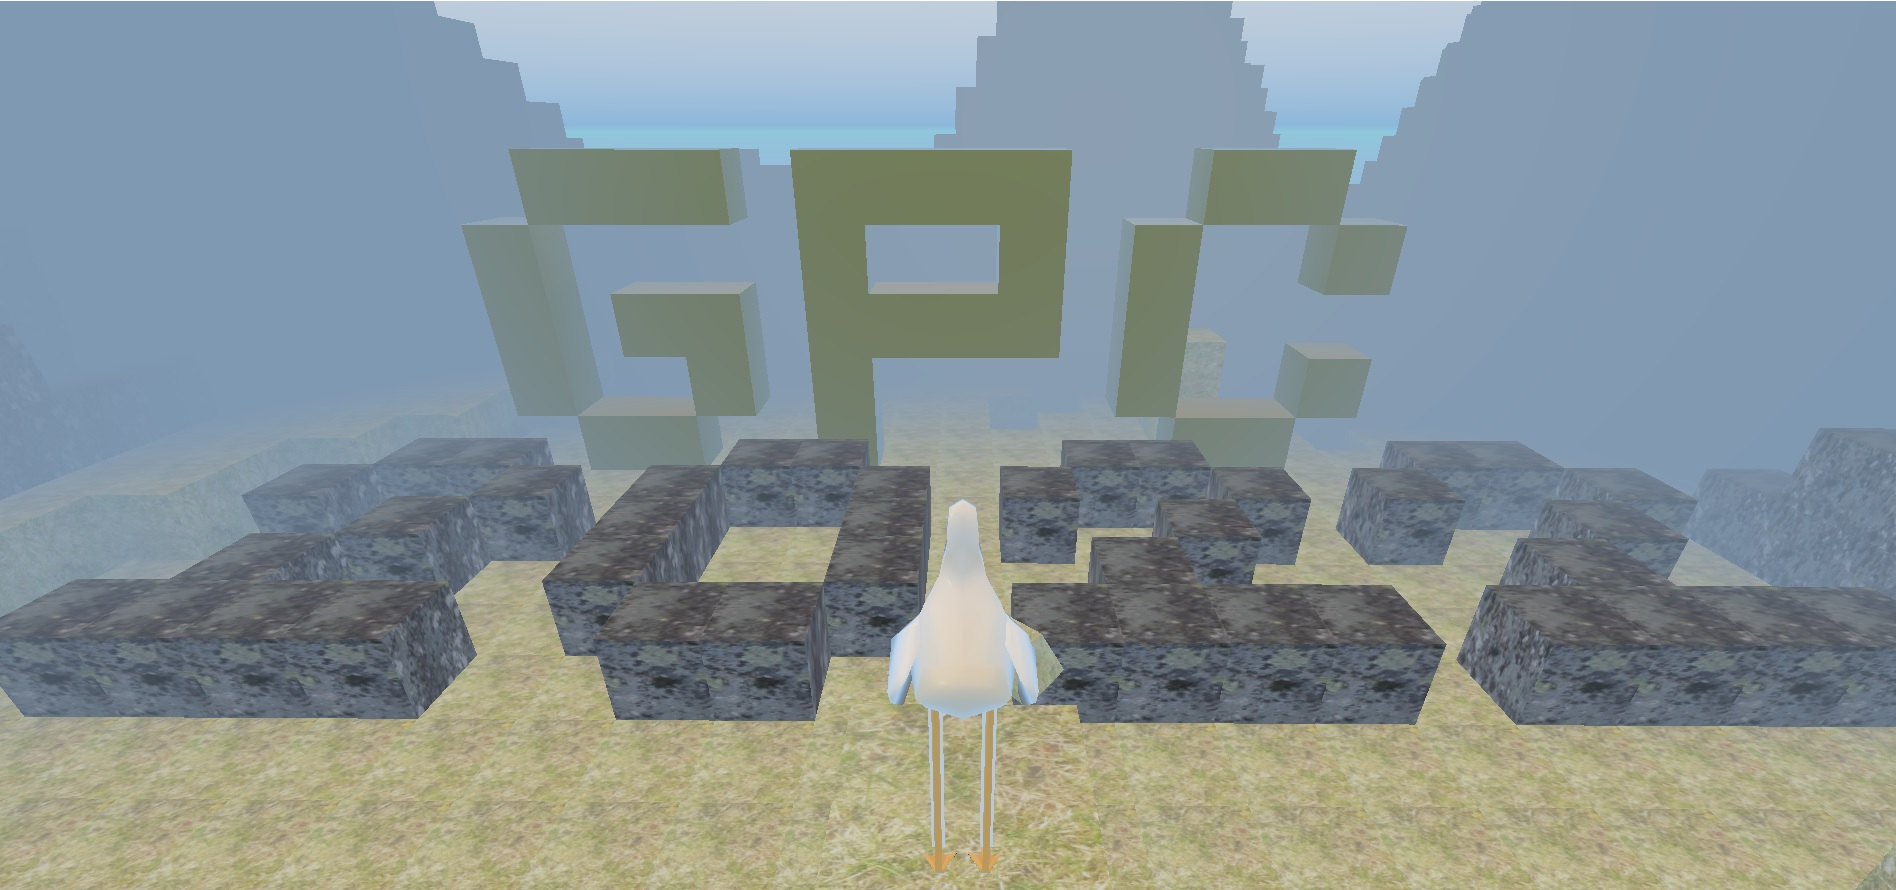
\includegraphics[scale=0.27]{gpc2022}
	\caption{A view of the game in third person mode}
\end{figure}
\tableofcontents

\section{Introduction}

\gamename\ is a game that features infinite procedural runtime terrain generation, the ability to create and destroy structures; and to save your creations. The game is built using Godot engine\cite{godotengine} version 3.4.4. It uses the GDScript language provided by Godot for the scripting.\par
The game is an exercise in procedural generation. The main goal of the game was to be a study in how to create 3D geometry on the fly that can be interacted with. Procedural generation provides great possibilities in terms of emergent gameplay and replay value.\par
The main goal of the project was to have procedurally generated terrain that can be edited during gameplay. Some features that can be found in similar games like an inventory or a crafting system are out of scope of this project.

\section{How to Play}
\subsection{Controls}
\begin{itemize}
	\item Mouse movement - Look around and rotate character
	\item Left mouse button - Place a block
	\item Right mouse button - Remove a block
	\item W,A,S,D keys - Move forward, left, backward and right respectively
	\item Space key - Jump
	\item 1, 2, 3, 4 keys - Change block type that will be placed
	\item C key - Change between first and third person camera perspectives
	\item Escape key - Open the pause menu
\end{itemize}
\subsection{Starting the Game}
The game can be started by pressing ``New Game" in the main menu. The game might take a few seconds to load. Additionally, a ``Load Game" button will be displayed in the main menu if you have previously saved a game. You can press the ``Load Game" button to continue from your previous save. Note that if you have previously saved your game, pressing ``New Game" will delete that save irreversibly.
\subsection{Saving the Game}
You can save your game by pressing the `Escape' key to open up the pause menu and pressing the ``Save Game" button. From the pause menu, you can also go back to the main menu by pressing the ``Main Menu" button, if you wish so.
\subsection{Building}
The player can place new blocks in their nearby environment. \autoref{fig:placebefore} demonstrates a view just before a player is about to place a block. When the first person mode is toggled, on the bottom right corner one can see the currently selected block type that will be placed in the environment. In the middle of the image, there is the block placement indicator, which shows the location where the new block will be placed. \autoref{fig:placeafter} shows the effect of placing the block in the environment. Additionally, a sound effect is played whenever a new block is placed.\par
Similarly, \autoref{fig:removebefore} shows an image of a situation before removing a block from the environment. \autoref{fig:removeafter} shows the same scene after pressing right click on the mouse, where a block has been removed. When removing blocks, a different sound effect is played.
\begin{figure}[hp]
	\centering
	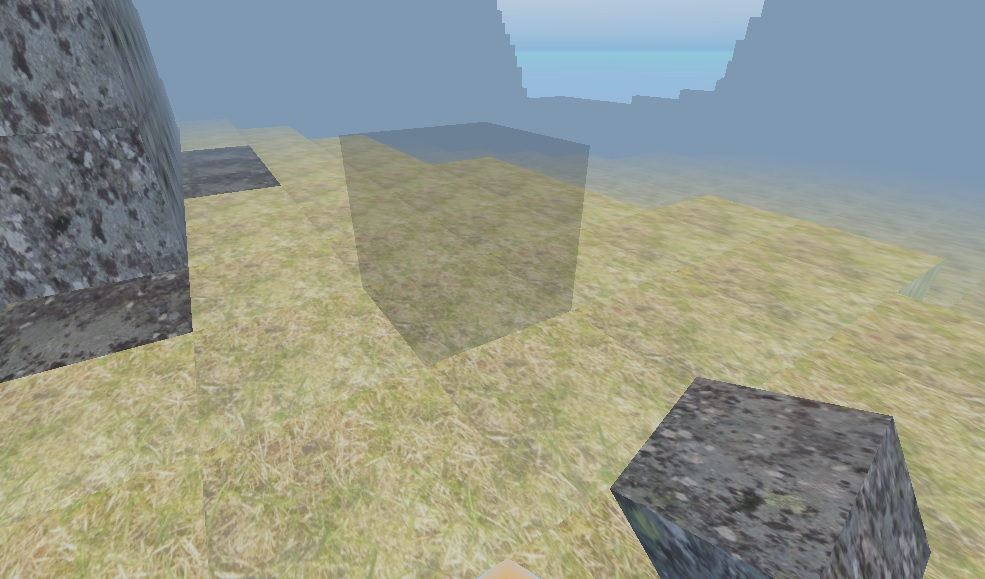
\includegraphics[scale=0.5]{placeblockbefore}
	\caption{View of the game before placing a block}
	\label{fig:placebefore}
\end{figure}
\begin{figure}[hp]
	\centering
	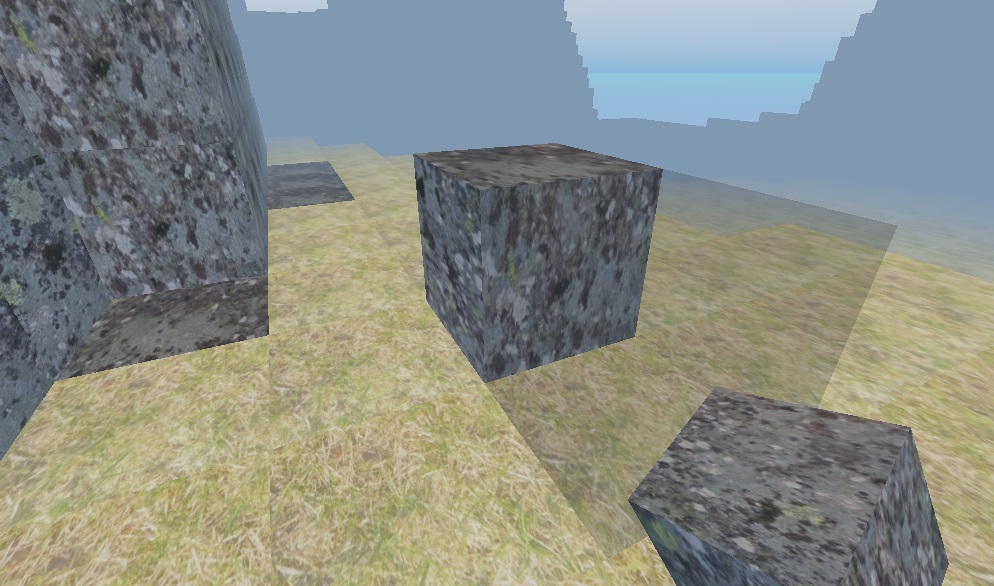
\includegraphics[scale=0.5]{placeblockafter}
	\caption{Same view after placing a block}
	\label{fig:placeafter}
\end{figure}
\begin{figure}[hp]
	\centering
	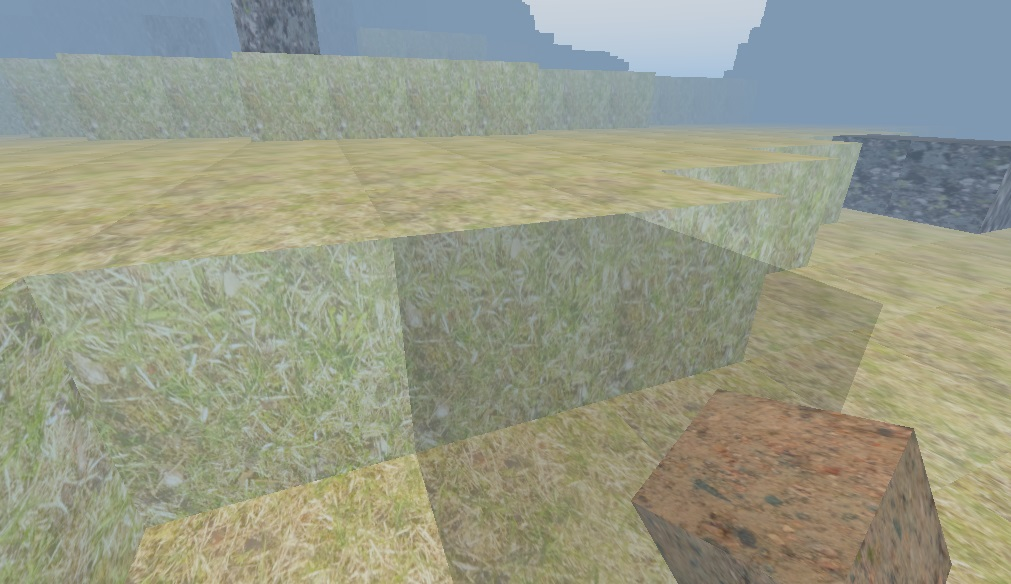
\includegraphics[scale=0.5]{removeblockbefore}
	\caption{View before removing a block}
	\label{fig:removebefore}
\end{figure}
\begin{figure}[hp]
	\centering
	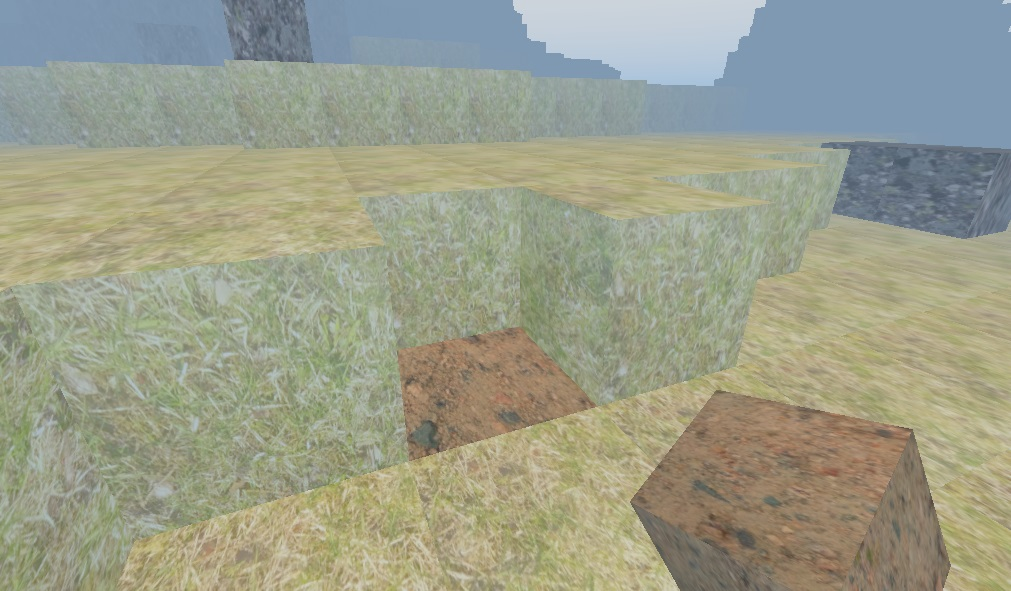
\includegraphics[scale=0.5]{removeblockafter}
	\caption{Same view after removing a block}
	\label{fig:removeafter}
\end{figure}
\subsection{Exploration}
\gamename\ features runtime procedural terrain generation. When you move around in the landscape, more and more land is being created around you for you to explore. To save memory, land that is far away from you will be unloaded, and the changes you might have made will be stored on the disk automatically. You press the ``space" key to jump. Jumping can come in handy when clearing obstacles and climbing mountains.
\section{Implementation Details}
\subsection{Godot Engine}
Godot is a feature-rich free and open source game engine suitable for producing 2D and 3D games alike. The main unit of structuring the game software in Godot is the Node. A Node represents some kind of entity in the game that has functionality. A Node may have child nodes, therefore they form trees. A tree of Nodes may be packaged as a self-contained and reusable unit called a Scene. A Scene, which is a tree of Nodes, may be instantiated as a Node itself. The tree of all currently active Nodes is called the Scene Tree. Adding and removing Nodes from the Scene Tree is how one controls which entities are currently present in the game.\par
Nodes that are in the Scene Tree can interact with each other with two ways. Nodes can call each others' functions that are defined for them. The functions that are defined for each Node are determined by their script. The other way Nodes can communicate is by using Signals. Signals are the Godot way of using the Observer pattern. A Node can have Signals defined and the script of the Node defines when the Signal is emitted. All other Nodes that are listening to that Signal of that Node will receive it, which will trigger a function in the receiving Node.\par
For more detailed information, please refer to the Godot engine documentation\cite{godotdocs}.
\subsection{Chunk}
The terrain is composed of cubic blocks that may have different textures. The cubes are further structured as a collection of cubes, which is called a Chunk. A Chunk keeps track of the current state of the blocks in a byte array of size 16x16x16, the value of the byte representing the type of a block in a certain location, with 0 byte being a special value that represents the absence of a block in that location.\par
In addition to the current state of the blocks within the Chunk, it has another byte array of size 16x16x16 which is used to keep track of the edits that have been made to the Chunk. In this array, a special byte value of 255 is used to represent a location that has not been edited by the player, with any other value being the type of the block which has been placed by the player to that specific location, or a value 0 if the player has removed a block from that location.
\subsection{Meshing}
The smallest unit used in meshing is the Chunk. That means that every time any block in a Chunk changes, the whole Chunk is remeshed. While some performance gains could be gained by identifying only the specific part of the Chunk that changed, and changing the mesh only in that part, that would greatly increase the complexity of the algorithm and therefore be more prone to bugs.\par
The meshing algorithm is simple. In brief, the byte array of block types in different locations of the Chunk is iterated and cube faces are added to the appropriate locations. The vertices of the mesh are kept track of in a hash table where a key is the type of a block and it points to an array of vertices. Each block location is checked if it is non-zero, which means that the location is non-empty. If it is non-zero, then check if it is either located in the edge of the Chunk or if it has any empty neighbours. Push vertices representing a cube face to the vertex array corresponding to the block type for those sides of the cube that fulfil those conditions. The vertex arrays are then used to generate the graphical mesh of the Chunk, and the appropriate textures are applied to the cubes based on which key their vertices were under. The vertex arrays under all of the keys are combined to form the collision mesh.
\subsection{Saving the Game}
The state of the player character is saved to a simple JSON file. However, saving of the state of the terrain is a much more complex matter that needs a more robust solution. For saving the edits made by the player to the terrain, the game uses the SQLite\cite{sqlite} database engine. The interface between Godot and SQLite is provided by the godot-sqlite\cite{godotsqlite} plugin.\par
The edits made to a Chunk are saved when the player chooses to save the game from the pause menu, or when the Chunk is unloaded because the player walked too far away from it. When attempting to save a Chunk, it is first checked for its dirtiness status. When a Chunk is initially loaded, the dirtiness flag is set to false. The flag is set to true only if the Chunk has been modified by the player since it was loaded. If the Chunk is not dirty, it does not need to be saved and it can be skipped. If the Chunk is dirty, then a new row is attempted to be inserted into the Chunks table that is created in the SQLite database when a new game is started. Each row of the Chunks table stores the coordinates of the Chunk and the diff array of the Chunk which represents the edits made by the player. The table has uniqueness constraints defined on the coordinates of the Chunk. The new row is inserted using an upsert\cite{upsert}. An upsert works like an insert if the new row does not violate a uniqueness constraint. If the new row violates the uniqueness constraint, then the existing row for the Chunk with the same coordinates is edited instead and the new diff array will replace the old one, but no new row is added to the table.
\subsection{Generating Terrain}
Terrain generation works in two modes, synchronous and asynchronous. The synchronous mode of terrain generation is used when the game world is initialized, because there must be some terrain under and immediately around the player when the game starts. However, after the game world is initialized and when the player moves around in the game world, the new Chunks are generated in the asynchronous mode. If Chunks were generated synchronously during playing, the game would pause for a while each time which would result in a poor playing experience. The algorithm used by synchronous and asynchronous modes for generating a single Chunk is the same, the only difference is that synchronous mode creates the Chunks immediately, while the asynchronous mode uses a separate worker thread.\par
The asynchronous mode of terrain generation is triggered when the player crosses a Chunk border. Each Chunk defines an Area. Area is a predefined Godot Node with represents a shape in the space of the game world, which in this case is the bounding box of the Chunk. When the player enters the Area, it sends a Signal to a Chunk manager. The Chunk manager, called "RollingChunks", keeps track of all the current Chunks that are loaded and is responsible for loading and unloading them. The list of Chunk coordinates which are located within a radius of the Chunk which player recently entered is compared with the list of Chunks that are currently loaded. If there are Chunks in that radius that are not yet loaded, their coordinates are pushed to a queue of Chunks that will be loaded asynchronously.\par
The queue is processed by a separate worker thread. The queue is implemented as a Godot array. Since using any operations on Godot arrays that modify their size is not thread safe\cite{arraysafe}, the queue array is always locked with a mutex when any items are queued or dequeued.\par
The procedurally generated terrain features of the Chunk are defined by sampling from smooth noise, specifically the OpenSimplexNoise\cite{opensimplex} which is provided natively by Godot. Each block location of the Chunk is iterated and the y-coordinate, corresponding to the height value of the block, is compared with the sample to determine if the block location is populated or not. Additionally, samples are drawn from several sources to determine the specific type of a populated block.\par
After the procedurally generated terrain features are determined, the SQLite database is queried to check if the Chunk has been edited by the player before. If the Chunk coordinates match a row in the Chunks table of the database, the diff array representing the edits made by the player is fetched and the diff is applied to the Chunk. The Chunk is then meshed and after that it is added to the game world. Unfortunately, the godot-sqlite plugin has a poor interface where it saves the result of the previous query to a global variable. This does not guarantee thread safety, so the reads from the database have to be locked with a mutex.\par
It might be in some cases possible to walk into a region of terrain that has not been loaded. To mitigate issues that this causes, each time a Chunk boundary is crossed, it is checked whether the Chunk that is entered into is loaded yet. If it is, the global coordinates of the Character are saved, since these coordinates should be safe to be in. If the Chunk is not loaded yet, the Character is teleported into the coordinates of the last entered loaded Chunk.
\subsection{Unloading Terrain}
Unloading Chunks works much like loading. The same Signal for entering a new Chunk that triggers loading new Chunks also triggers unloading faraway Chunks. A list of Chunks that are outside a certain radius is generated and those Chunks are unloaded. Each Chunk is first checked for dirtiness flag. If the Chunk is marked as dirty, it is first saved to the database. Then, the Chunk is removed from the game world using the Godot built in method \textit{queue\_free}. The radius for unloading faraway Chunks is a bit larger than the one for loading new Chunks. Otherwise, if the player were to constantly move back and forth in a Chunk border, it would result in Chunks being constantly loaded and unloaded, which could lead to poor performance. The unloading of Chunks is a much faster operation than the loading of Chunks, therefore it is simply done synchronously.
\subsection{Adding and Removing Blocks}
The main problem when adding a block is to determine which Chunk the new block should be in. When the player attempts to add a block, a ray is casted from the character to the environment. If the ray collides with a Chunk, it may not be the correct Chunk if the location where the block should be added is on the edge of the Chunk. Therefore, the solution calls for a more sophisticated method than simply raycasting to a Chunk and telling the Chunk to add a block to itself.\par
Although the Chunk can only modify its own blocks, given the global coordinates of the ray, it can tell what is the correct Chunk that the block should be added to. The Chunk transforms the global coordinates to local coordinates and based on those it can tell if the block is contained within it. The Chunk will tell the Character Node the correct Chunk coordinates where the block needs to be placed in. The Character will then emit a Signal to the "RollingChunks" Chunk manager to add the block. The Chunk manager will fetch the Chunk matching to the coordinates and add the block to the desired location.\par
Removing a block works similarly. The main difference is that the block the casted ray is pointing to will be the one that is desired to be removed. Therefore it is guaranteed to be in the correct Chunk and there is no need for the machinery of seeking the correct Chunk.
\subsection{Character Physics}
Character physics are modeled after the 1996 PC game \textit{Quake}\cite{quake}. A blog article\cite{strafe} was used as a reference for creating similar character movement experience. This method of modeling character physics should provide for smooth movement. The player can control the movement direction of the character while in air, hopefully providing a less frustrating experience while jumping due to not feeling locked in.\par
The method is based on keeping track of the character velocity and applying acceleration to the desired direction in each frame based on the player input. Friction is applied to the character if they are touching the ground or a wall. There are maximum velocity constants for ground acceleration and air acceleration defined separately. If the velocity in the next frame would exceed the maximum velocity, the speed is limited to the corresponding maximum. If the character is in the air, some downward acceleration is applied which models gravity. Jumping on the other hand is achieved by applying some upward acceleration to the current velocity if the character is touching the floor. In each frame, the character is moved by the amount and to the direction of the velocity vector. The velocity vector is used as the input to Godot built in function \textit{move\_and\_slide\_with\_snap} which handles collisions and sliding along colliding surfaces automatically.
\subsection{Diagram of the Structure}
The diagram \autoref{fig:arch} shows a sketch of how the game is structured. Solid directed arrows denote an ownership relationship. Dotted directed arrows mean that a Signal is sent between Nodes of those types. Dashed directed arrows denote that the Node interacts with the other Node, but does not own it. Dashed undirected arrow means using a plugin. Dashed blank arrow denotes a source of input.
\begin{figure}[h]
	\centering
	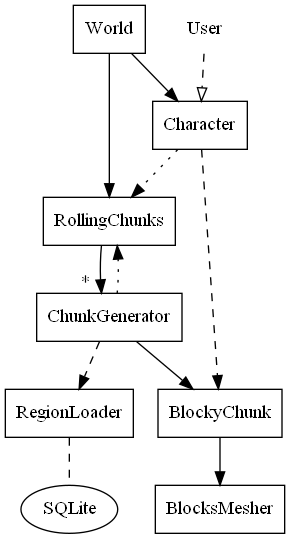
\includegraphics[scale=0.5]{arch}
	\caption{Sketch of the Structure of the Game}
	\label{fig:arch}
\end{figure}
\section{Testing}
The project unfortunately does not include automated testing. Testing of various features was accomplished during development by printing various values to console. I have since deleted most of the debug outputs. Some of the issues that were debugged using this style were:
\begin{itemize}
	\item The amount of Chunks loaded when crossing the Chunk border, to make sure the Chunk unloading is working as expected and that there is an upper bound to how many Chunks can ever be loaded at once (seems to be about 120)
	\item The physics jitter bugs were debugged simply by printing the character location in each frame
	\item The vertices of the Chunk mesh, to verify whether it includes all of them, to investigate a bug where not all of them were being drawn
	\item When the character is crossing the Chunk boundary, to make sure the Signal for crossing the boundary is actually fired
\end{itemize}
\section{Known Bugs}
\begin{itemize}
	\item The game is known to sometimes crash randomly
	\item Blocks sometimes cannot be placed from certain angles
	\item It is possible to fall through ground when placing a block where you are currently standing in
\end{itemize}
\begin{thebibliography}{9}
\bibitem{godotengine}
Godot Engine home page, \url{https://godotengine.org/}
\bibitem{godotdocs}
Godot Docs, \url{https://docs.godotengine.org/en/stable/index.html}
\bibitem{sqlite}
SQLite, \url{https://www.sqlite.org/index.html}
\bibitem{godotsqlite}
Godot-sqlite Github repo, \url{https://github.com/2shady4u/godot-sqlite}
\bibitem{upsert}
SQLite Docs upsert, \url{https://www.sqlite.org/lang_UPSERT.html}
\bibitem{arraysafe}
Thread-safety of Godot Arrays, \url{https://docs.godotengine.org/fi/stable/tutorials/performance/threads/thread_safe_apis.html#gdscript-arrays-dictionaries}
\bibitem{opensimplex}
OpenSimplexNoise in Godot Docs, \url{https://docs.godotengine.org/fi/stable/classes/class_opensimplexnoise.html}
\bibitem{quake}
Quake, 1996, in Wikipedia, \url{https://en.wikipedia.org/wiki/Quake_(video_game)}
\bibitem{strafe}
Adrian Biaglioni, "Bunnyhopping from the Programmer's Perspective", \url{https://adrianb.io/2015/02/14/bunnyhop.html}
\end{thebibliography}
\end{document}